%\begin{noindent}
\begin{markdown}
# Zielkriterien

## Hardwarespezifikation

Um den Lift zu steuern, wird eine SPS von Siemens verwendet. Die SPS kann fix verbaut werden, da der Lift in einem Gebäude verbaut wird, wird die SPS keinen Umwelteinflüssen ausgesetzt. Zudem ist anzunehmen, dass immer dieselbe Temperatur herrscht. Die SPS benötigt 5 Eingänge und 7 Ausgänge. Von den 7 Ausgängen werden mit 5 Schützen angesteurt, um in weiterer Folge die Motoren zu steuern. Mit den anderen Zwei Ausgänge werden Lampen angesteuert, welche signalisieren, wohin der Lift fährt. Aus sicherheitstechnischen Gründen wurde für den Lichtschranken (S1) ein Öffner verwendet und für die Türen (Q3, Q2, Q1) ein Schließer. Die zwei Endschalter (H1, H2) signalisieren, wenn der Lift in einem Stock angekommen ist.

\begin{figure}[h!]
    \centering
    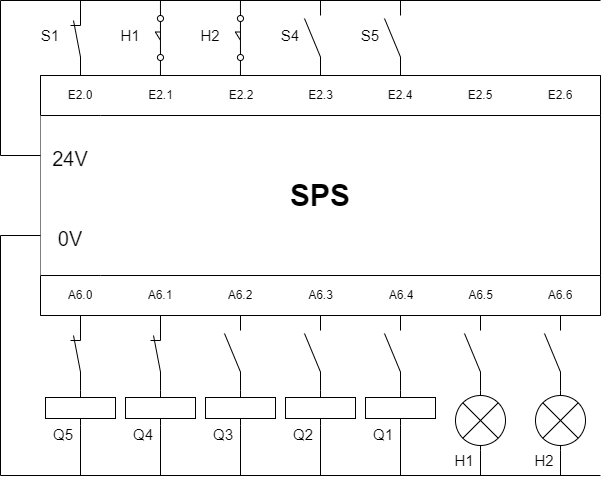
\includegraphics[width=0.8\textwidth]{./images/Anschlussschema.png}
    \caption[Anschlussschema der SPS]{Anschlussschema der SPS}
\end{figure}

### Human Machine Interface (HMI)

Es gibt in jeder Etage, in die der Lastenlift fährt, einen Druckknopf. Dieser Knopf ist dazu da, um den Lift zu rufen und die Türen zu öffnen. Im Lift gibt es zwei Druckknöpfe, wobei einer dafür dient, um in den unteren Stock zu fahren. Der andere dient dazu, um in den oberen Stock zu fahren. Zudem können mit den Knöpfen die Türen geöffnet werden. Im folgendem Bild werden alle Endschalter, Sensoren, Leuchten und Stockwerke abgebildet.

- hS1 und hS2 stellen Lampen dar _(sie zeigen an, in welcher Etage sich der Lift befindet)_
- SEndS1 und SEndS2 stellen den unteren und oberen Endschalter dar _(sie erkennen, ob der Lift im unterem oder oberen Stockwerk angekommen ist)_
- sMoveToS1 und sMoveToS2 stellen Taster im Lift dar _(sie werden zur Navigation des Liftes verwendet)_
- sSendToS1 und sSendToS2 stellen Taster außerhalb des Liftes dar _(sie werden zum Rufen des Liftes verwendet)_
- sDoorBlock stellt den Lichtschacht dar _(dieser wird benötigt, um die Türen zu stoppen, falls diese blockiert wird)_ 
- aDoorS2 und aDoorS1 stellen die jeweiligen Türen in den Stockwerken dar
- aDoorElev stellt die Liftdür dar

\begin{figure}[h!]
    \centering
    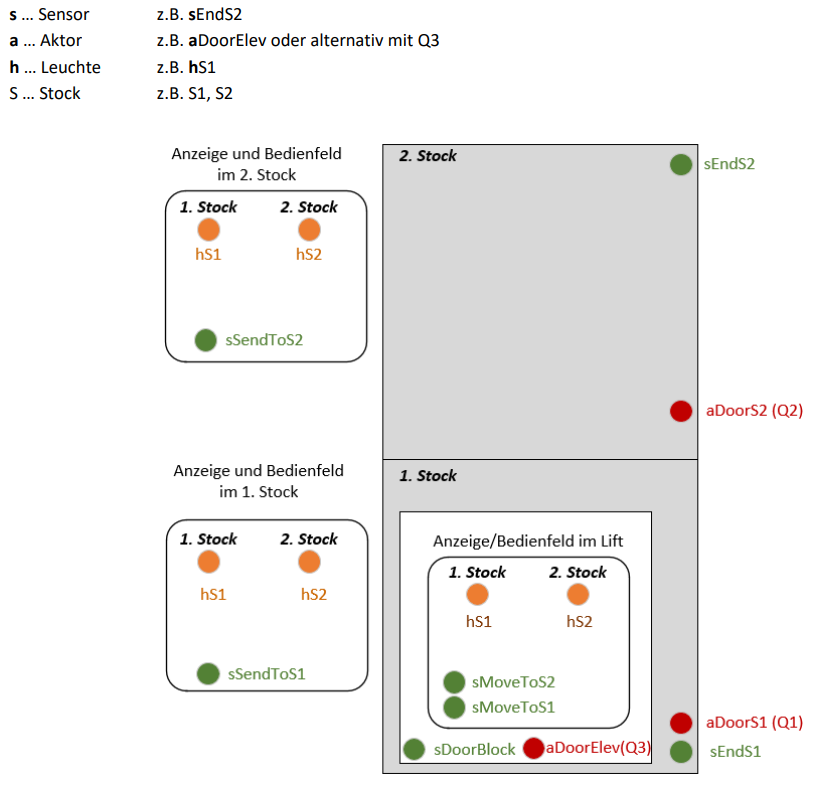
\includegraphics[width=0.8\textwidth]{./images/Skizze.png}
    \caption[Skizze des Lastenliftes]{Skizze des Lastenliftes mit Sensoren, Aktoren und Signalleuchten}
\end{figure}

Alle Zustände und Zusammenhänge können aus der folgenden Zustands- und Zuordnungstabelle abgelesen werden:

\begin{figure}[h!]
    \centering
    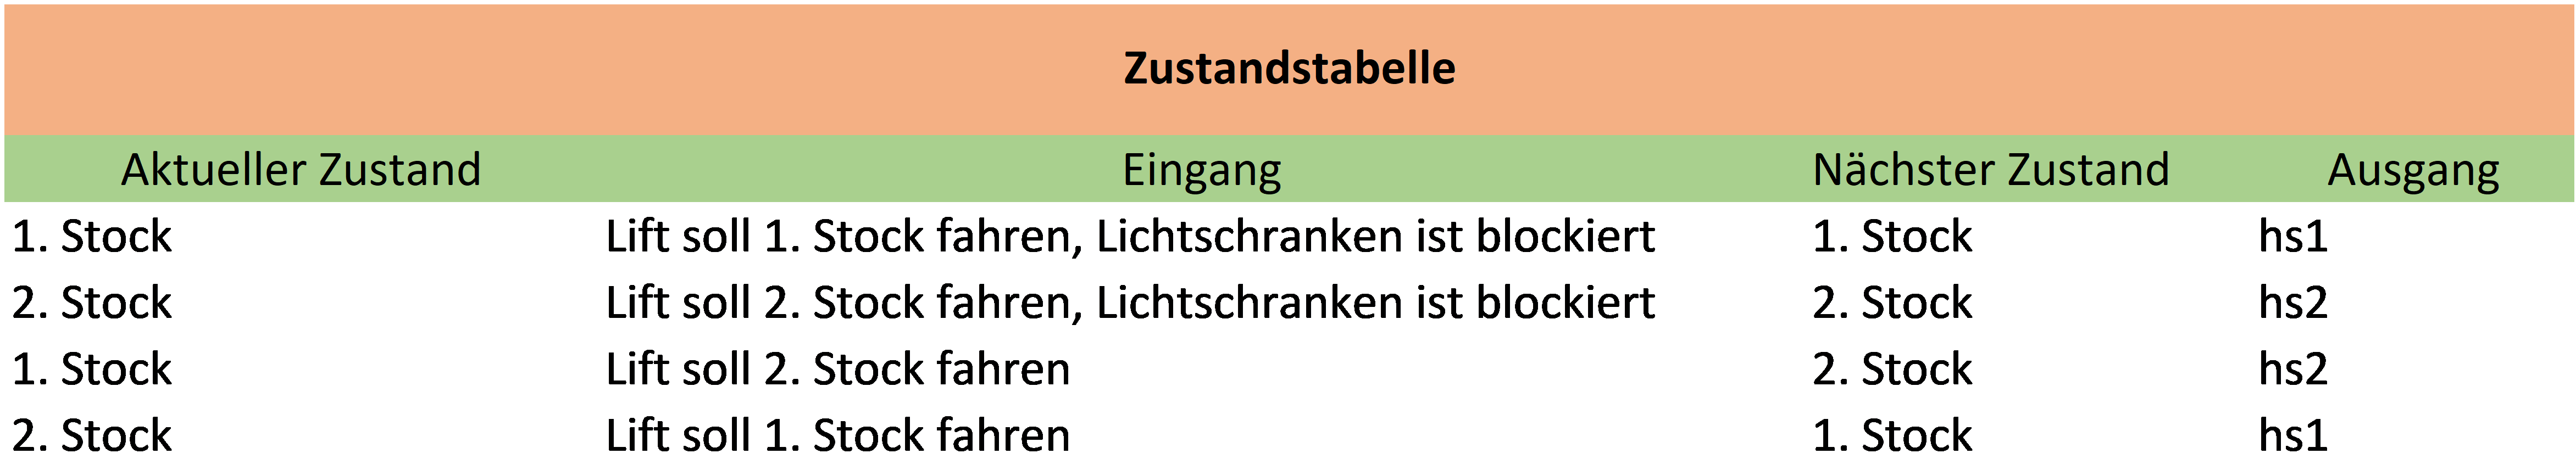
\includegraphics[width=0.8\textwidth]{./images/Zustandstabelle.png}
    \caption[Zustandstabelle]{Zustandstabelle}
\end{figure}

\begin{figure}[h!]
    \centering
    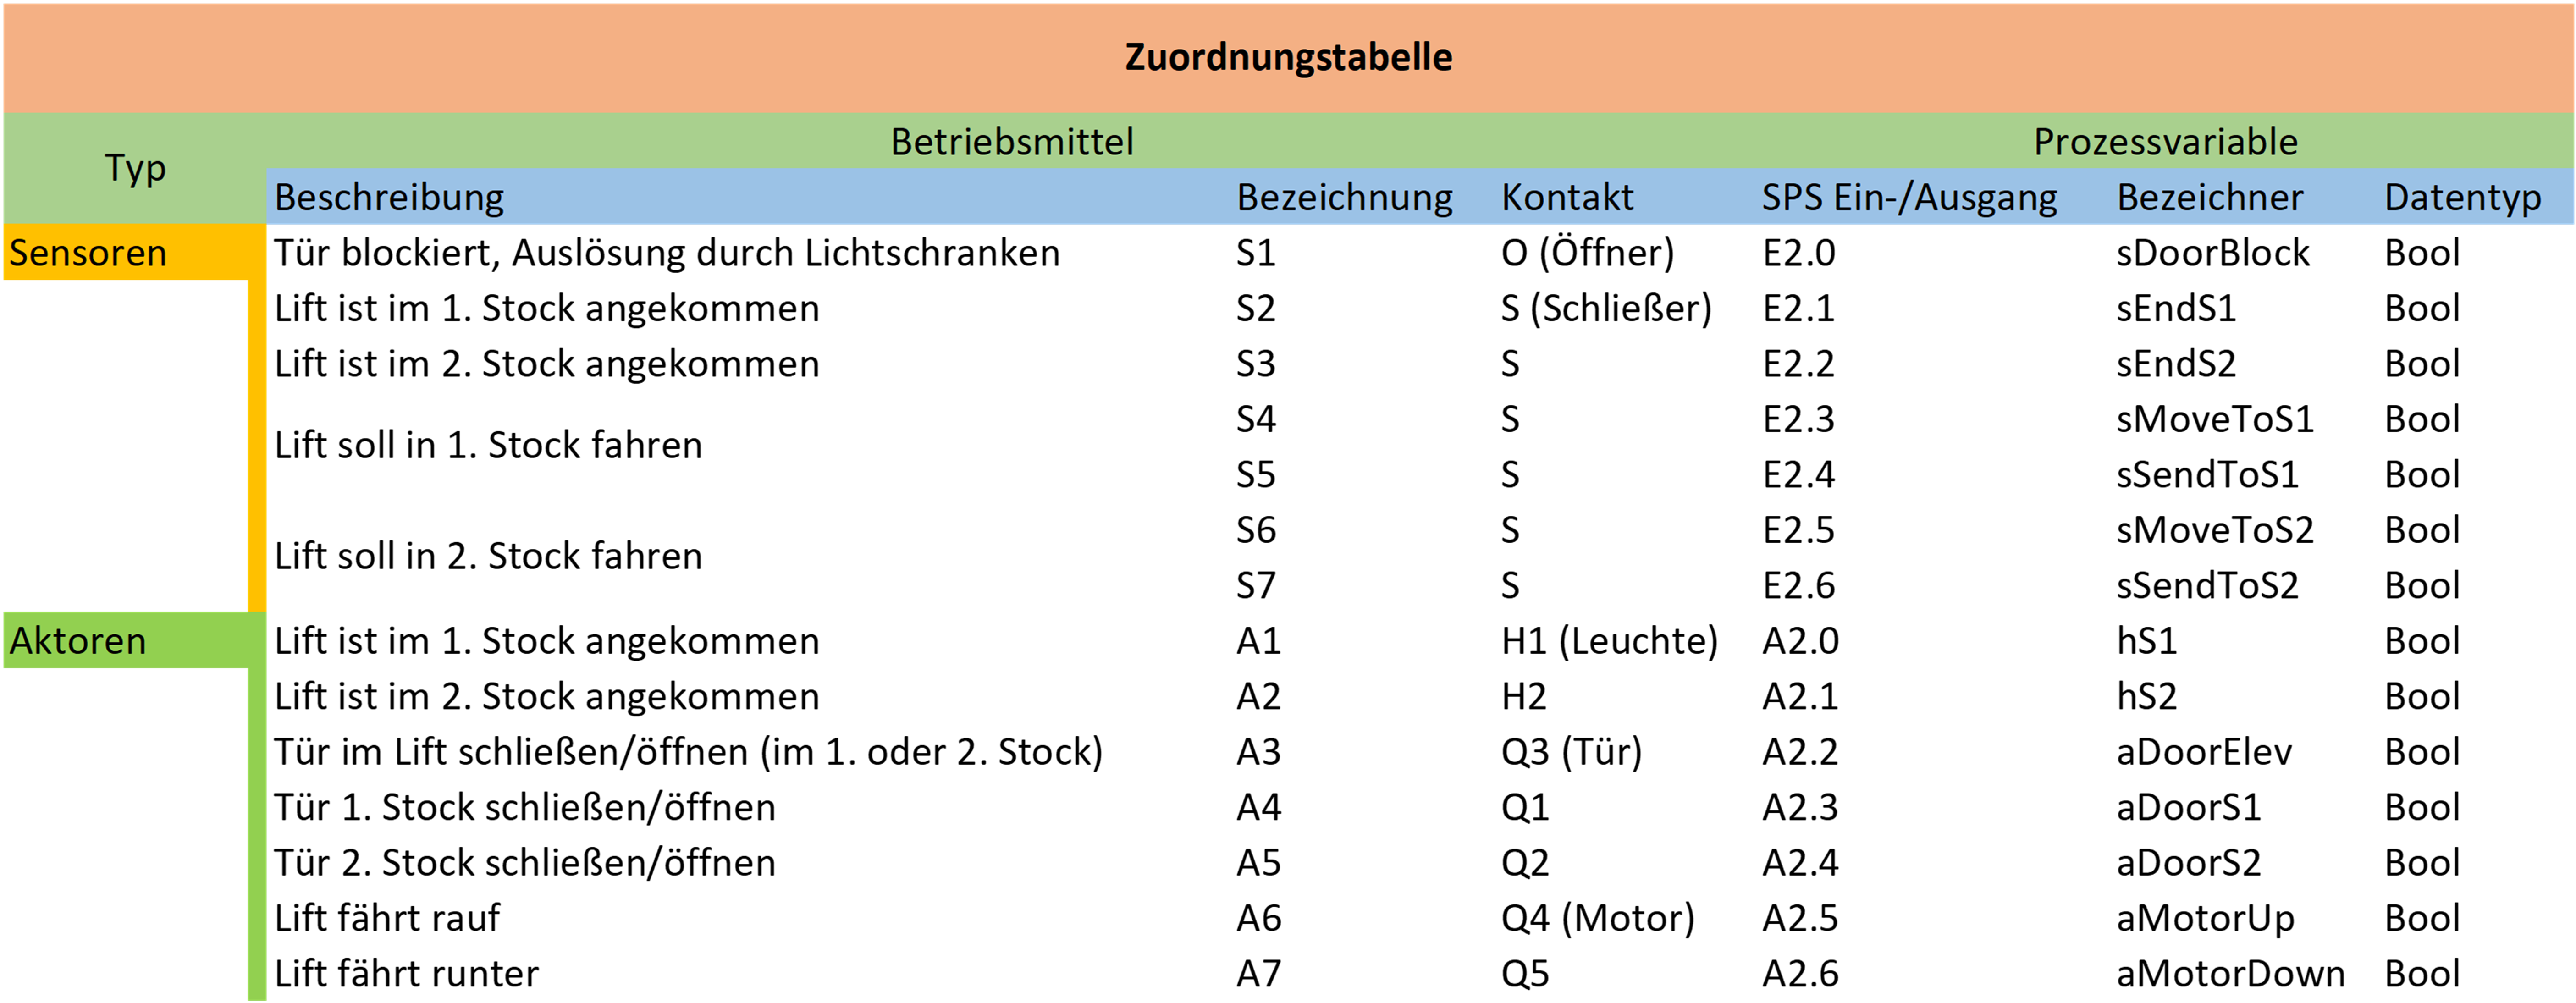
\includegraphics[width=\textwidth]{./images/Zuordnungstabelle.png}
    \caption[Zuordnungstabelle]{Zuordnungstabelle}
\end{figure}

## Softwarespezifikation

Das Programm wird in Automation Studio mit Hilfe von STL (Strukturiertem Text) programmiert. Es wird auf Basis von States umgesetzt. Zudem werden Timer benötigt, um die Lifttüren Zeitbasiert zu schließen. Zudem müssen sich, wenn die Lichtschranke blockiert wird, die Lifttüren öffnen, da es sonst zu Sicherheitsrisiken kommen kann. 

### Human Machine Interface (HMI)

Der Lift wird im Einzelschrittbetrieb betrieben und kann nur unter bestimmten Situationen in einen anderen Betriebsmodus wechseln, wie zum Beispiel bei Wartungsarbeiten.

## Test und Industrialisierung

Für alle Sensoren und Aktoren wurden Technisch hochwertige Produkte ausgewählt, um die Sicherheit und die Funktionalität zu gewährleisten. Um sicher zu stellen, dass es nach der Inbetriebnahme zu keinerlei Störungen kommt, wurde ein maximales Gewicht festgelegt, welches der Lift befördern darf.

## Maschinensicherheit

Um den Lift in Betrieb nehmen zu dürfen, ist ein CE-Kennzeichen von Nöten. Deshalb müssen alle notwendigen Normen eingehalten werden.
\end{markdown}
%\end{noindent}